\begin{center}
  \centering 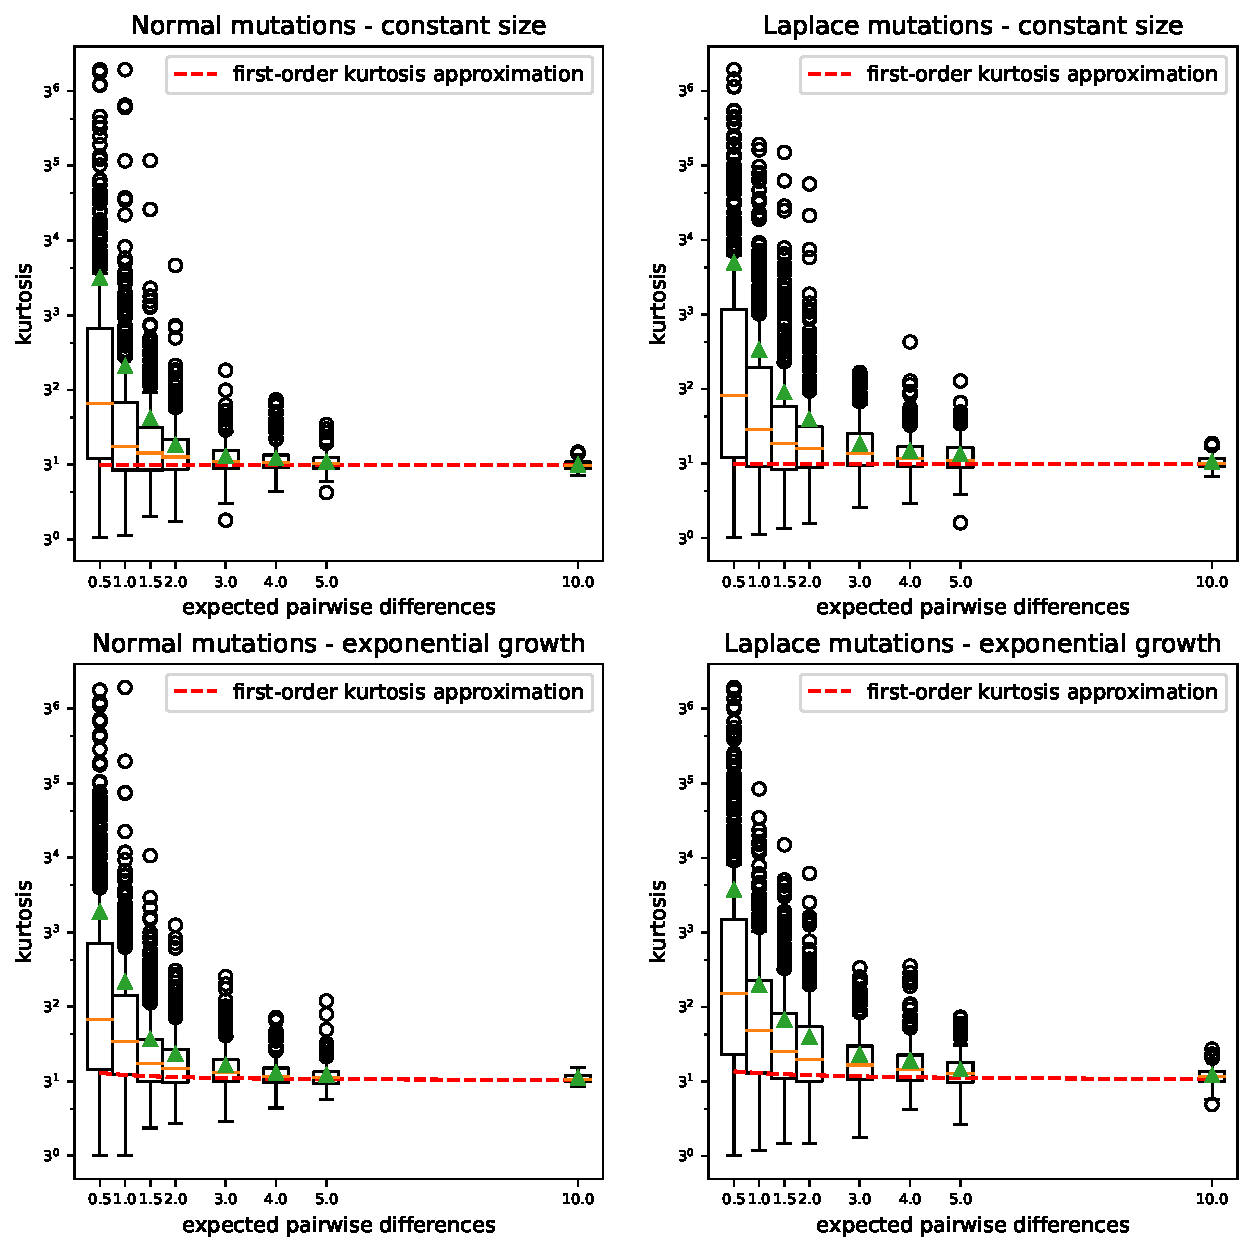
\includegraphics[width=\textwidth]{figures/kurt_sim.pdf}
  \captionof{figure}{\small The distribution of the population kurtosis under
    different levels of sparsity, mutational kernels, and demographies. The
    sparsity is varied by changing the expected number of pairwise differences
    at sites affecting the trait. Normal and Laplace distributions of mutational
    effects are compared. A constant size population is compared to an
    exponential growth scenario with growth rate equal to the reciprocal of the
    final effective population size. Green triangles denote the mean kurtosis.
    The dashed red lines give the first order approximation to the expected
    kurtosis given in equation \ref{eq:firstord}.}
  \label{fig:kurtsim}
\end{center}
Entire populations were simulated using msprime \citep{Kelleher2015} and
mutations were assigned effects from a zero-centered normal or Laplace
distribution. The effective population size and mutation rate were kept constant
and the expected number of pairwise difference was increased by increasing the
number of loci affecting the trait.

A first order approximation to the kurtosis is
\begin{equation}
    \label{eq:firstord} 
\kappa_Y^{(1)} = 3 + \frac{m_4/m_2^2 \frac{\CCC}{\E[\mathbbm{T}_{2,2}]}} {L \T \E[\mathbbm{T}_{2,2}]
    + m_4/m_2^2 \frac{\BBB}{\E[\mathbbm{T}_{2,2}]}}.
\end{equation}
Although this expression suggests that the expected $\kappa_Y$ will be greater
than under normality when external branches are longer ($\E[\mathbbm{T}_{4,4}] >
\frac{1}{6}\E[\mathbbm{T}_{3,4}] + \frac{1}{9}\E[\mathbbm{T}_{2,4}]$) and less
than under normality when they are longer ($\E[\mathbbm{T}_{4,4}] <
\frac{1}{6}\E[\mathbbm{T}_{3,4}] + \frac{1}{9}\E[\mathbbm{T}_{2,4}]$),
simulations show that the approximation is actually quite poor (Figure
\ref{fig:kurtsim}).
%%% Local Variables:
%%% TeX-master: "short_report.tex"
%%% End:
